\section{Modularization}

% -----------------------------------
\subsection{Modularization Motivation}

\begin{frame}
\frametitle{Why Modularization}
\begin{itemize}
\item Growth management
\pause
\item Software quality improvement
\pause
\item Facilitating add-ons
\pause
\item Separate third party libraries
\pause
\item Optional Components
\end{itemize}
\end{frame}

% -----------------------------------
\subsection{Modularization Implementation}

\begin{frame}
\frametitle{Module sizes}
\center
\begin{center}
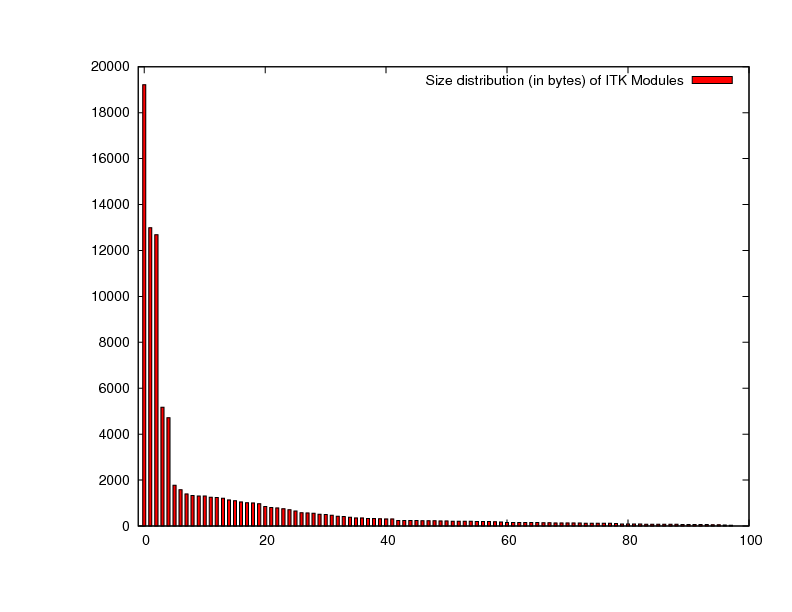
\includegraphics[height=0.8\textheight]{../Art/moduleSizePlot.png}
\end{center}
\end{frame}

\begin{frame}
\frametitle{Module sizes (no third party modules)}
\center
\begin{center}
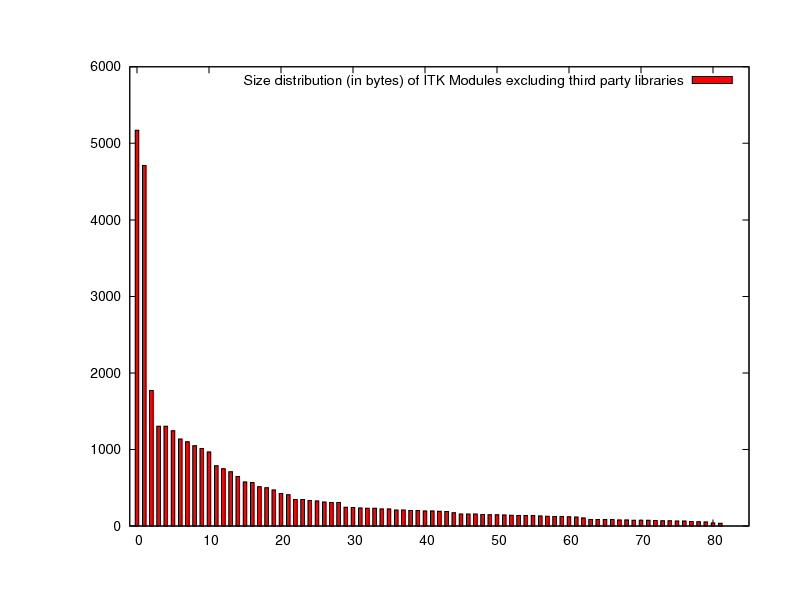
\includegraphics[height=0.8\textheight]{../Art/moduleSizePlotNoThirdParty.png}
\end{center}
\end{frame}

\begin{frame}
\frametitle{Visualize dependencies among modules}
\center
\begin{center}
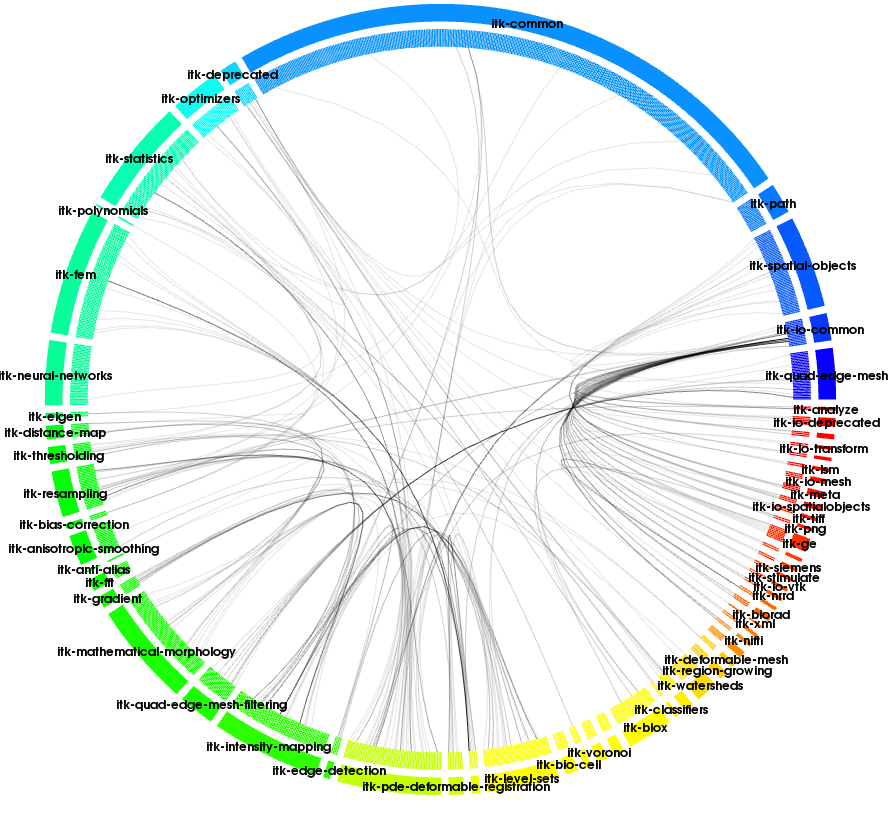
\includegraphics[height=0.8\textheight]{../Art/moduleDependency.png}
\end{center}
\end{frame}

\begin{frame}
\frametitle{ITK Module Grouping}
\begin{itemize}
\item  12 groups, 98 modules and counting
\pause
\item  Group by module functionalities
\pause
\item  Archiving modules in groups
\pause
\end{itemize}
\end{frame}

% -----------------------------------
\subsection{Add Your Own Module}

\begin{frame}
\frametitle{How to add a module into ITK}
\begin{itemize}
\item Where to put a module (categorization)
\pause
\item How to construct a module (CMake magic)
\end{itemize}
\end{frame}


\begin{frame}
\frametitle{Modularization checklist}
\begin{itemize}
\item  Module categorization: module group, module name
\pause
\item  Directory hierarchy: include, test, src
\pause
\item  CMake configuration: CMakeLists.txt
\pause
\item  Module dependency: itk-module.cmake
\pause
\item  Add tests, \href{http://www.vtk.org/Wiki/ITK/Git/Develop/Data\#Workflow}{\textcolor{red}{\underline{add testing data}}}
\pause
\item  Documentation
\end{itemize}
\end{frame}


\begin{frame}
\frametitle{A toy example: ITKRAT}
\begin{itemize}
\item  itkRobustAutomaticThresholdImageFilter(RAT)
\pause
\item  An external module: ITKRAT
\end{itemize}
\end{frame}


\begin{frame}
\frametitle{More information on Modularization}
\begin{itemize}
\item  Details about ITK Modularization can be found at \href{http://www.itk.org/Wiki/ITK\_Release\_4/Modularization}{\textcolor{red}{\underline{Wiki Page}}}.
\end{itemize}
\end{frame}
